\documentclass[11pt,a4paper]{article}
\usepackage{float}
\usepackage[utf8]{inputenc}
\usepackage[left=1.5cm,right=1.5cm,text={19cm,26cm},top=1.5cm]{geometry}
\usepackage{graphicx}
\usepackage{rotating}
\usepackage{hyperref}
\usepackage[english]{babel}

\begin{document}
    \noindent
    \Large{\textbf{Documentation of Project 2 Implementation for IPP 2022/2023}}
    \normalsize \\
    Name and surname: Matyáš Strelec \\
    Login: \verb|xstrel03|


\section{Introduction}

The \verb|interpret.py| is a script which takes a source file of an IPPcode23 program, which has been checked and converted to an XML representation
by a parser which was implemented in the 1st project, and interprets the source, therefore running the code.


\section{Prototype design pattern}

For the implementation using OOP, I chose the Prototype design pattern\cite{prototype}. Here, the \verb|Instruction| class is 
a prototype for all the sub-classes for each separate instructions. This achieves abstraction of
implementation, as well as unifying the execution method of each instruction.


\section{Implementation}

The program is contained in the \verb|interpret.py| file, most of the code is structured into classes.
Important parts of the code have explanatory comments.


\subsection{Main function}

The main function is simple, as it only instantiates the necessary classes and uses them to begin 
executing the program itself. The respective classes are described in following sections.


\subsection{\texttt{InputFiles}}

The class is initialized by creating a parser using \verb|argparse|, from which it reads the needed
arguments, also printing the help message if prompted. As the script supports the input or source file both from a file using the command line argument, reading from \verb|stdin| also must be supported. Therefore, the 
correct source for both is decided and the files are opened. Errors while opening or reading the files are also handled here.


\subsection{\texttt{Xml}}

The class takes the input file in form of an XML representation of IPPcode23. Using the \verb|ElementTree| 
library, XML is easily parsed. The needed attributes of the XML are checked, returning respective errors if
necessary.

The opcode is read and it's expected arguments are loaded as an array from the \verb|Helper| class,
for each argument, the order, type and value is checked. If they're correct, a object is created which
represents the argument, and this object is appended to the instruction.

Using the \verb|eval()| function, an instance of the class with the same name as the opcode is created. The instructions are then ordered by the order tag. The \verb|get_instructions()| method is used to return them.


\subsection{\texttt{Prog}}

The most important class is \verb|Prog|, where the interpretation happens. When initializing, an empty program
is created, with instructions, variable storage in frames and the stack and the control flow.

The \verb|run()| method takes given instructions and fills the list. First, all labels are collected to prevent
their redefinition. Then, the interpretation begins from the first instruction.

The class contains many useful methods that are used when working with variables. The storage system of frames
is used here. For reading and writing into variables, they must be defined first. If they are defined, first,
the local frame gets searched, then the temporary frame, and finally the global frame. If the variable is not
present, an error gets returned.


\subsection{\texttt{Instruction}}

Each instruction has the \verb|opcode|, \verb|args| and \verb|program| attributes, as well as the \verb|execute()| function. \verb|Args| is a list of \verb|Arg| objects, and \verb|program| is the
instance of \verb|Prog| class currently executing the code.

For every opcode, there's a sub-class which has it's own \verb|execute()| method, according to the Prototype
design pattern.\cite{prototype}. The execution implementation varies by instruction, but each one acceses
it's argument using \verb|get_argN()| function of the \verb|Instruction| class. The \verb|program| argument is
an instance of the \verb|Prog| class, storing all information about the executed code needed for the 
instruction to work with variables and program's control flow . 

 
\subsection{\texttt{Arg}}

\verb|Arg|, and it's many sub-classes are a representation of data in IPPcode23. They contain the \verb|data|
attribute, which can be the numerical value for integers or text for string.

These objects are the arguments of functions in IPPcode23, and are stored as attributes of their corresponding
instructions.

For a visual representation of class inheritance refer to the UML diagram\ref{fig:uml}.


\subsection{\texttt{Helper}}

The \verb|Helper| class contains methods and attributes that are used through the whole program. There are
two static methods, \verb|string_escape()| and \verb|error_exit()|, a list of opcodes, and a dictionary of 
their expected arguments.

\verb|String_escape()| takes a string and converts all corresponding escape sequences to their respective
characters. It checks if the escape sequences are valid and returns the result string.

\verb|Error_exit()| is used to print debug information when exiting with an error. It prints the given
error and it's given exit code. If the method was called from a running program, which was passed as an
argument, it also prints the instruction and position in code.

\verb|Opcodes| are a list of permitted operation codes. \verb|ExpectedArgs| are used to determine if an
argument that was given when reading the source code has the correct type.

\vspace{\fill}

\bibliographystyle{plain}
\bibliography{readme2}

\eject \pdfpagewidth=297mm \pdfpageheight=80mm
% \textwidth=297mm
\newpage

\vspace*{\fill}

\begin{center}
    \begin{figure}
        \centering
        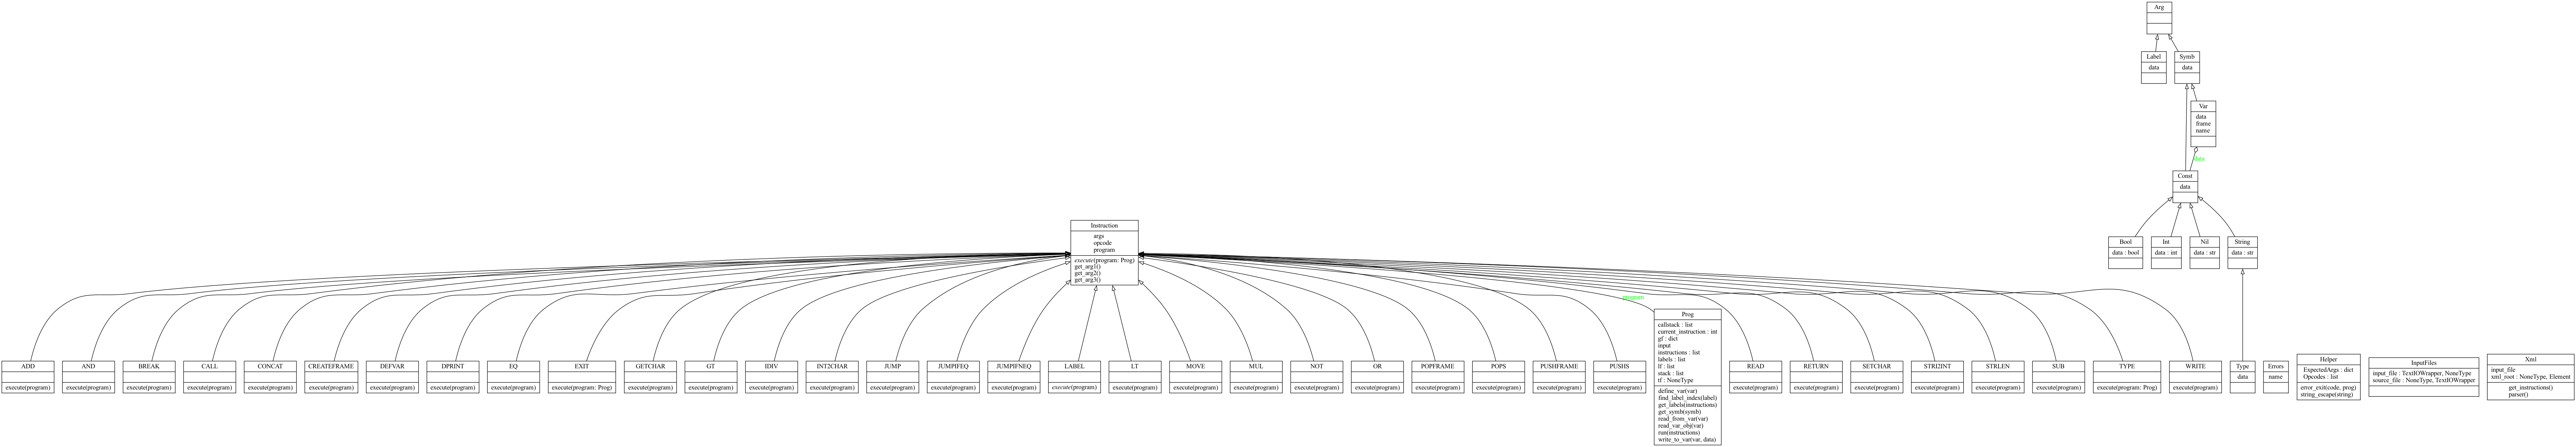
\includegraphics[width=0.9\pdfpagewidth]{classes.png}
        \caption{UML diagram}
        \label{fig:uml}
    \end{figure}
    \end{center}

\vspace*{\fill}

\end{document}